\begin{figure}[p]
\centering
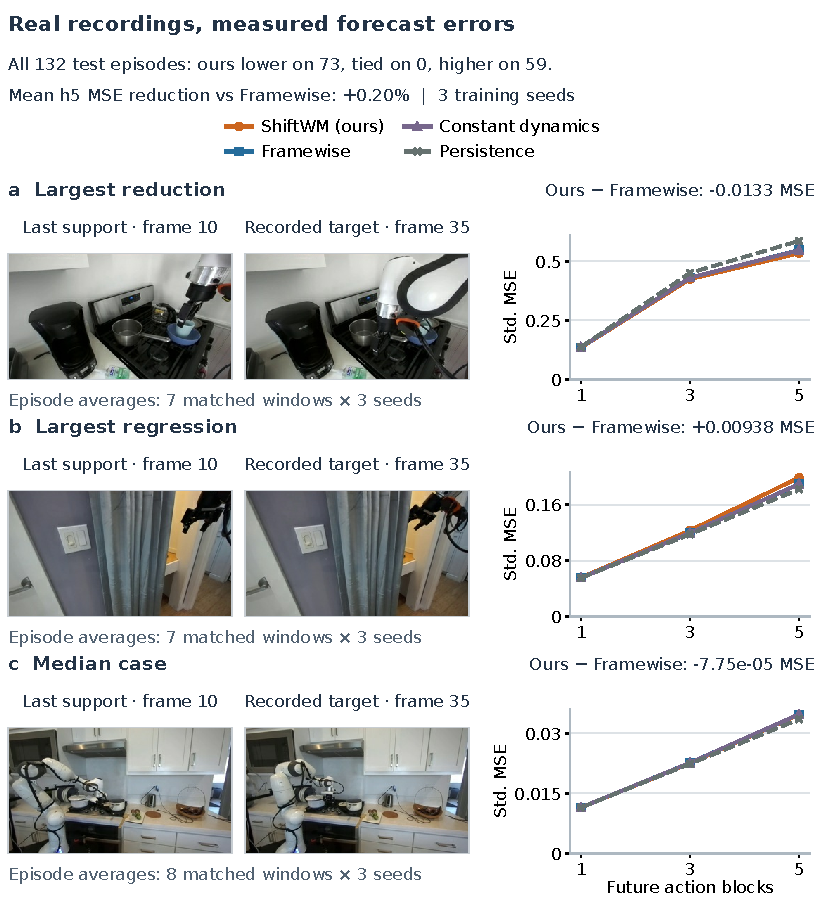
\includegraphics[width=\linewidth]{generated/real_video/comparison_recorded_droid.pdf}
\caption{\textbf{Real DROID recordings with measured feature-forecast errors.}
The primary held-out camera-1 population is summarized above three deterministically
selected episodes: the largest reduction, the largest regression, and an episode nearest the median in ours-minus-Framewise h5 standardized MSE
(ties by episode ID).
Each image pair shows the last observed support frame and final recorded query
target from the first evaluated window; these are actual photographs, not decoded
predictions. Each curve averages all evaluated windows of that episode, then all
three training seeds, at the three measured horizons. Panel y-axis ranges differ;
methods within each panel share the same axes. Curves show point means; the full-test paired 95\% h5 MSE-difference interval includes zero. The models observe three support
frames and recorded commands; persistence repeats the last support feature and
requires no training. The displayed images illustrate a recording and do
not localize the aggregate error or establish why a method wins. Selection is
outcome-conditioned and is not a frequency estimate: all-test counts and mean
reduction are reported above. Error reductions are feature-forecast differences,
not robot-control success or evidence of an identified causal mechanism.}
\label{fig:real-video-comparison}
\end{figure}
